This section will cover the internal logic of the compiler.

\subsection{Listeners}
As mentioned in section~\ref{subsubsec:compilertools} our compiler is based on the ANTLR parser generator.
More specifically, the compiler is written in C\#.
While ANTLR was originally designed for Java, considering the individual expertise of the group members,
using the C\# version was the more convenient option.

ANTLR also provides an alternate pattern to the classical visitor pattern, the listener pattern.
"The biggest difference between the listener and visitor mechanisms is that
listener methods are called by the ANTLR-provided walker object, whereas
visitor methods must walk their children with explicit visit calls. Forgetting
to invoke visit() on a node’s children means those subtrees don’t get visited." ~\cite{ANTLRReference}.

Therefore, to mitigate some of the disadvantages we have due to our smaller group size, we can rely on the listener pattern
and only write the specific listener methods we care about while ignoring the specifics of walking the rest of the tree.

Notably, to facilitate the usage of the listener pattern, there were some minor changes introduced in the final grammar.
For example, the rule \lstinline{ifblock} was broken down into two parts: \lstinline{ifblock} and \lstinline{ifheader}.
This has the advantage of allowing us to create separate listener methods for when the lexer exits
the header part of the if statement, immediately allowing us to parse and translate it.
Without separating the rules, we would have to manually traverse the context, the latter would result in a
more fragile code base.

We have created multiple listener classes ~\ref{fig:listener_class_diagrams}, all of them inheriting from the base class: \lstinline{LatticeBaseListener}.
This approach creates a more readable codebase compared to having a single listener class with all the relevant
listener methods.
Moreover, some classes implement the same listener method but behave differently, based on the compiled code.
For example both \lstinline{VariableListener} and \lstinline{GraphListener} implement the \lstinline{ExitVardecl}
However, \lstinline{GraphListener} only modifies the output when a graph is declared, while \lstinline{VariableListener}
handles all other variable declarations.

\begin{figure}[H]
    \centering
    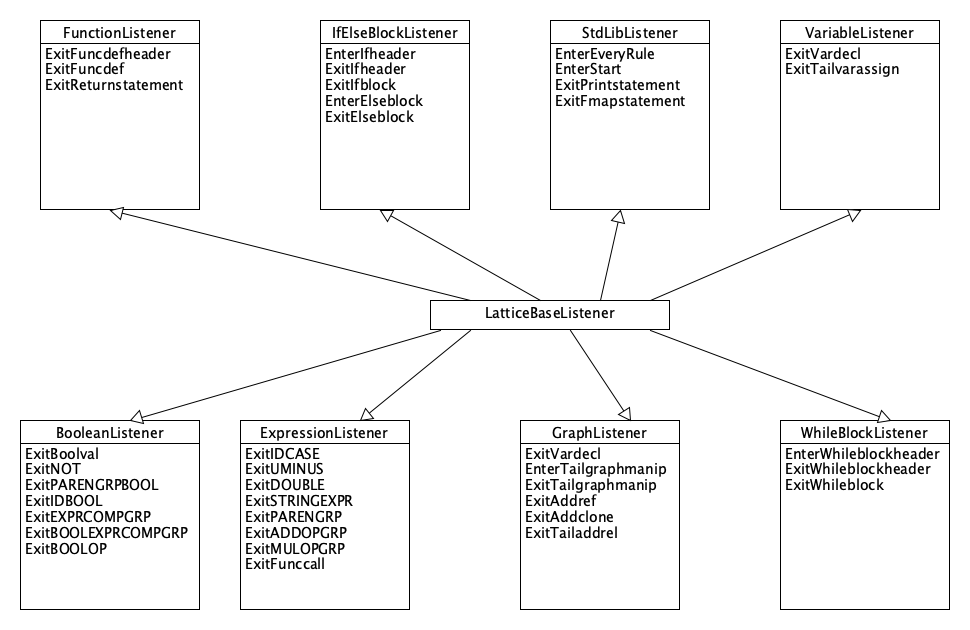
\includegraphics[width=12cm]{figures/implementation_section/listeners}
    \caption{Listener classes implemented in the compiler}
    \label{fig:listener_class_diagrams}
\end{figure}

\subsection{Context Management}
Like most other programming languages, Lattice also deals with contexts.
For instance functions are independent blocks of code, separate from the main structure.
The main focus of Lattice are the graphs, they also behave as independent contexts.
Nodes defined within a graph block are unique to that specific context.

In terms of the compiler's implementation, the main component responsible for context management is the
\lstinline{ContextManager} static class.
It has multiple responsibilities, namely:

\begin{itemize}
    \item Maintains a stack of all the open contexts.
    \item Provides an interface for the rest of the codebase to interact with the context stack (open, close, get).
    \item Keeps track of the innermost graph context.
    \item Maintains a dictionary of all declared functions.
\end{itemize}

Each context class inherits from the abstract class \lstinline{Context} (figure: ~\ref{fig:contexts}).
This base class implements the shared logic of all contexts, such as a symbol table for variables (implemented as a dictionary)
and a dictionary of all subordinate contexts.

\begin{figure}[H]
    \centering
    \includegraphics[width=12cm]{figures/implementation_section/contexts}
    \caption{Context classes}
    \label{fig:contexts}
\end{figure}

The \lstinline{IfBlockContext} and the \lstinline{WhileBlockContext} are essentially featureless implementations
of the \lstinline{Context} base class.
However, implementing them as unique classes allows future expansion, and some level of type safety within C#.

An interesting note about the \lstinline{FunctionContext} is that the \lstinline{Parameters} property is implemented
as a queue.
Classical structures such as linked lists and arrays do contain the original ordering of the items added,
therefore they would be sufficient to store the parameters.
However, the benefit of using a queue instead, is that it forces us, the developers to always consider the ordering of
the parameters - which is especially beneficial when performing semantic checks on the function signature.
These parameters are also folded into the \lstinline{_variables} list to ensure that the semantic check performed
when accessing them as variables do pass.

The \lstinline{GraphContext} heavily expands the base class' functionality.
As the name suggests it is responsible for managing the graph operations.
The main functionality is related to the management of nodes and relationships, detailed in subsection ~\ref{subsec:nodes_and_relationships}

\subsection{IO operations}
Compiling to Python introduces a few unique challenges.
Due to the nature of its syntax, the compiler has to be mindful of the indentation.

The interface for the actual code output is the static class \lstinline{GlobalFileManager} (figure ~\ref{fig:global_file_manager})).
It can output both to the stdout and to a specified file.

Listener methods may call the \lstinline{Write} method to output code to the specified channel.

It also implements the \lstinline{Indent} and \lstinline{Outdent} methods, which as the names suggest are responsible
for maintaining correct indentation.
In reality, the indentation is simply tracked in the form of an integer.

Whenever a listener calls the \lstinline{Write} method, the class checks whether the previous parameter string ended
in a line feed, if so, the output string is prepended with the appropriate amount of whitespaces.

This check is necessary to give the listeners the flexibility to output code in smaller chunks, instead of forcing
them to only write complete lines.

In action, using the \lstinline{GlobalFileManager} is as shown in listing ~\ref{lst:compiler_global_file_manager}.

\begin{lstlisting}[caption={Using the GlobalFileManager to enter an else block},captionpos=b, label={lst:compiler_global_file_manager}]
    public override void EnterElseblock(LatticeParser.ElseblockContext context)
    {
        OpenNewIfElseContext();
        GlobalFileManager.Outdent();
        GlobalFileManager.Write($"else:{Program.NewLine}");
        GlobalFileManager.Indent();
    }
\end{lstlisting}

\begin{figure}[H]
    \centering
    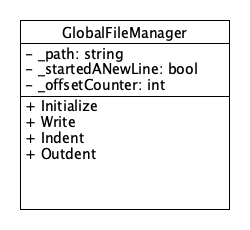
\includegraphics[width=6cm]{figures/implementation_section/globalfilemanager}
    \caption{GlobalFileManager}
    \label{fig:global_file_manager}
\end{figure}

\subsection{Lattice Types, Variables and Expressions}
A large section of semantic checks in Lattice are related to type safety.
Lattice, however, has relatively few types, and has no mechanism to expand the available types.
Therefore, the compiler maintains a hardcoded enum of the available types.

Whenever a type is parsed, it gets translated to the corresponding \lstinline{LatticeType} enum value.
Since there is no evaluation of expressions during compilation, the values are stored as strings.
For example, consider this simple Lattice code snippet: \lstinline{int a = 5+5;}.

While it could technically be evaluated at compilation time to the integer 10, there is no clear benefit in doing so.
Therefore, the Variable object will simply contain the string form of the expression \lstinline{5+5}.

Expression objects behave in a very similar manner.
They only need to know the string form of the expression (in Python form) and its evaluation type.
With these two properties, the compiler is capable of performing semantic checks, and code generation.

\begin{figure}[H]
    \centering
    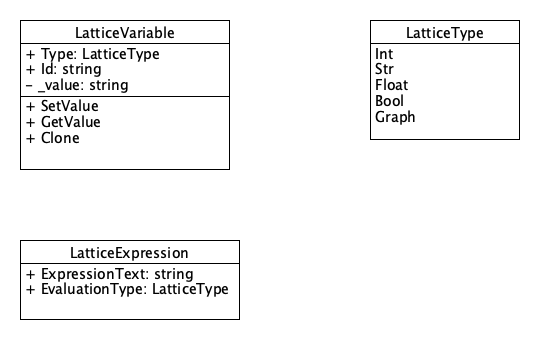
\includegraphics[width=6cm]{figures/implementation_section/varexprtype}
    \caption{Class Diagram for LatticeExpression, LatticeVariable and LatticeType}
    \label{fig:exprs-vars-types}
\end{figure}

The grammar does make a distinction between boolean and other expressions, but the compiler can in fact
treat these two types the same, simply setting the correct evaluation type for the object.

When a Lattice expression is parsed, it may pass through multiple listener methods before it gets output.
For example, consider the following expression: \lstinline{(true || boolvar)&&some_boolean_function()}.
This expression would in fact pass through 6 listener methods (based on the grammar rules).

Since the tree walking is an implicit action, we could not rely on return values.
Therefore, as suggested by the ANTLR reference manual, we used a stack based approach.

Listing ~\ref{lst:expression_listener_excerpt} shows an excerpt on how the stack is used to construct a complete expression.
Since the IDCase (reference to a variable) is an atomic operation, there is no need the check the stack for other expressions.
Instead, the method simply checks whether the referenced variable exists in the current context, and pushes the
ID as an expression to the stack.

On the other hand, a parenthesis rule is meaningless without a subordinate expression.
So the method first pops the last expression from the stack,
creates a new expression object of the last expression wrapped in parentheses and puts it back on the stack.

\begin{lstlisting}[caption={ExpressionListener class excerpt},captionpos=b, label={lst:expression_listener_excerpt}]
    public override void ExitIDCASE(LatticeParser.IDCASEContext context)
    {
        var id = context.ID().GetText();
        var variable = ContextManager.GetCurrentContext().GetVariable(id);
        var expression = new LatticeExpression(id, variable.Type);
        ListenerHelper.SharedListenerStack.Push(expression);

    }

     public override void ExitPARENGRP(LatticeParser.PARENGRPContext context)
    {
        var expression = PopExpressionFromStack();
        var parenExpression =
            new LatticeExpression($"({expression.ExpressionText})", expression.EvaluationType);
        ListenerHelper.SharedListenerStack.Push(parenExpression);
    }
\end{lstlisting}

Finally, if for example, the expression was used in a variable assignment, the \lstinline{ExitVardecl} method
implemented in the \lstinline{VariableListener} (listing ~\ref{lst:compiler_var_assign}) class will pop the expression from the stack and assign it
as a value to the relevant variable.

\begin{lstlisting}[caption={VariableListener class excerpt},captionpos=b, label={lst:compiler_var_assign}]
    public override void ExitVardecl(LatticeParser.VardeclContext context)
    {
    var type = LatticeTypeHelper.StringToLatticeType(context.type().GetText());
    if (type == LatticeType.Graph) return;

    var id = context.ID().GetText();
    var newLatticeVar = new LatticeVariable(id, type);
    if (ListenerHelper.SharedListenerStack.TryPop(out var latticeExpression))
    {
        AssignVarValueAndPrintPythonCode(ref newLatticeVar, latticeExpression);
    }
    ContextManager.GetCurrentContext().DeclareVariable(id, newLatticeVar);
}
\end{lstlisting}

\subsection{Nodes and Relationships} \label{subsec:nodes_and_relationships}

In the current state of the project, the \lstinline{Node} class is just a featureless inheritance of the \lstinline{LatticeVariable} class.
This is because, nodes essentially behave exactly as a variables, with the distinction that nodes are specific to graph contexts.

There are two types of relationships implemented in the compiler (shown on figure ~\ref{fig:relationships}).
\lstinline{DirectedRelationship} and \lstinline{UndirectedRelationship}.
Both of them inherit from the base abstract class \lstinline{Relationship}, which implements the shared behavior,
namely cost and label.

The difference between the two concrete implementations corresponds to the mathematical definition of edges.
The class \lstinline{DirectedRelationship} has a successor and a predecessor node, while \lstinline{UndirectedRelationship}
contains a pair of nodes in a non-particular order.

\begin{figure}[H]
\centering
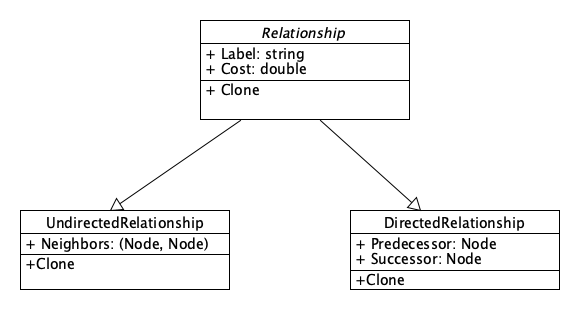
\includegraphics[width=12cm]{figures/implementation_section/relationships}
\caption{Class Diagram for Relationships}
\label{fig:relationships}
\end{figure}


\subsection{Inline Python Using Lexer Interjection}
A useful feature we have implemented is the option to include native Python code directly in Lattice.
This feature is made possible by ANTLR's channel system.

It allows us to send some lexer input to a separate channel, away from the rest of the input.
Normally it's used to ignore things like comments.
For instance, in our G4 file, comments are defined as such: \lstinline{MULTILINE_COMMENT   : '/*' .*? '*/' -> skip;}
where skip is an alias for a dead channel.

However, leveraging the same system, we defined the following rule: \lstinline{PYTHON: '<PYTHON>' .*? '</PYTHON>' -> channel(99);}
where any text between the tags \lstinline{'<PYTHON></PYTHON>'} are sent to channel 99 (an arbitrary number).

We then overrode the default \lstinline{LatticeLexer} generated by ANTLR (listing ~\ref{lst:custom_lattice_lexer}).
In our custom lexer, whenever a token is detected on channel 99, the token (which is the entire Python string)
gets enqueued in a static queue.

\begin{lstlisting}[caption={Excerpt from the class CustomLatticeLexer},captionpos=b, label={lst:custom_lattice_lexer}]
    public override IToken Emit()
    {
        if (Channel == 99)
        {
            var tokenText = Text;
            Text = null; // clear the buffer
            var token = base.Emit();

            //write out type python code
            ListenerHelper.LexerInterjects.Enqueue(StripPythonTag(tokenText));

            return token;
        }
        else
        {
            var token = base.Emit();
            var tokenText = Text;

            return token;
        }
    }
\end{lstlisting}
Finally, in the \lstinline{StdLibListener} class, we override the \lstinline{EnterEveryRule} method, to immediately
output out any enqueued Python code received from the lexer (listing ~\ref{lst:stdliblistener}).

\begin{lstlisting}[caption={Excerpt from the class StdLibListener},captionpos=b, label={lst:stdliblistener}]
    public override void EnterEveryRule(ParserRuleContext context)
    {
        while (ListenerHelper.LexerInterjects.Count > 0)
        {
            var interject = ListenerHelper.LexerInterjects.Dequeue();
            GlobalFileManager.Write(interject);
        }
    }
\end{lstlisting}

This approach has the benefit of being outside the language's grammar, removing the need to implement the entire Python
CFG.

However, it's important to note that since the interjects are outside the grammar, they can't be used freely in place
of normal Lattice code.
For example, the following piece of code is syntactically incorrect: \lstinline{int a = <PYTHON>foo()</PYTHON>}

Moreover, any inline Python code is outside the normal syntactic, semantic, and indentation checks.
Therefore, using them may result in invalid Python code generated.
\subsection{Testing}
To ensure that our compiler functions correctly we must construct a test suite that ensures valid lattice code compiles
correctly, and that invalid lattice code is appropriately handled.
Exhaustively testing language features is unsolvable, and language components are too interoperable to realistically
construct unit tests (no language components will realistically exist in a vacuum).
Our approach will largely involve focusing on target code snippets and matching them to concrete examples - this will
allow us to build regression tests to ensure that language changes do not affect established working code.
The unfortunate effect of this approach is that it leaves code open unexpected exploitations, our only defence against
this will be to attempt to create tests that logically could expose flaws (heuristically based on personal experience).

In this section we will explore the unit tests that we believe are sufficient to cover the language.
Our format for unit testing will be to have a section of lattice code, and expect a direct 1:1 translation to
python code - for report visualisations, we will write the translations as comments in python.
For the purpose of brevity, our examples may condense more than one test into a single block of code - this is not
desirable in real world testing as it makes it harder to narrow down a single point of failure.

\subsubsection{Variables and Expressions}
Our first test will be to ensure variable declaration and re-declaration - we can construct similar tests to test for
proper type checking.

\begin{lstlisting}[caption={Testing that variable declaration and type checking work},captionpos=b, label={lst:lattice-typing-test}]
int x = 5;                  // x = 5
int y = x + 5;              // y = x + 5
str y = 10;                 // error
bool z = x < y              // z = x < y
str y = "test";             // y = "test"
int z = "test" + y          // error
str x = "newtest";          // error - x already defined
\end{lstlisting}

These tests would continue for each combination of types and expression operators.
Unfortunately, even such a set of permutations is not infallible, as we see very unpredictable issues even in mature
languages such as Python~\cite{PythonIssue}.

\subsubsection{Branching Structures}
As the structures we test become more complex, we find that our tests need to become more creative, here we will
cover the tests we build to ensure the validity of loops, if/else statements, and functions.

Firstly we build tests for simple branching, which we translate directly, avoiding issues with dangling else statements
is avoided by relying on the Python compilation.
In contrast, ``hanging'' else statements should be accounted for.

\begin{lstlisting}[caption={Testing if-else statements},captionpos=b, label={lst:lattice-if-else-test}]
int x = 0;                  // x = 0
if (x < 5) {                // if x < 5:
    print "1";              //     print("1")
}
else {                      // else:
    print "2";              //     print("2")
}
else {                      // should error, currently ignored
    print "5"
}
\end{lstlisting}

For continuations of these tests, we check for all expression permutations within the if statement, and ensure the
syntactic invalidity of missing characters (such as unclosed brackets).

Next we move on to looping; as we are compiling to a language that already supports looping, our main concern for while
loops is to ensure that indentation and the while loop expression itself remain intact.

\begin{lstlisting}[caption={Testing while loops},captionpos=b, label={lst:lattice-while-loop-test}]
int x = 0;                  // x = 0
while (x < 5) {             // while x < 5:
    x = x + 1;              //     x = x + 1
}                           //
print x;                    // print(x)
\end{lstlisting}

Similarly to if-else statements, we then create tests for combinations of expressions, and ensure that syntax errors
are caught.

Lastly we move on to functions, our main departure from the previous examples in this section is that we require a
syntactic check to ensure that the return statement complies with what has been defined.

\begin{lstlisting}[caption={Testing functions},captionpos=b, label={lst:lattice-function-test}]
def str function1 (str x) {  // def function1(x):
    return x;                  //    return x
}
def str function2 (int x) { // error (mismatching types)
    return x;
}
str x = function1("test");    // x = function("test")
str y = function1(5);          // error (mismatching types)
\end{lstlisting}

As always, we then create permutations for each type, and a set of syntax errors.

\subsubsection{Nodes and Relationships}
Our tests for this section will focus on correct translation of creating references and opening contexts.
This is the first structure that we explore that doesn't have a direct translation, our focus on the translation will
be to ensure that operations done within a context affect the correct graphs outside.

\begin{lstlisting}[caption={Testing graphs},captionpos=b, label={lst:lattice-graph-test}]
graph g1{                   // g1 = Graph()
    int x = 5;              // x = 5
    ref x;                  // g1.add_nodes(x=Node(5)
    graph g2 {              // g2 = Graph()
        int y = 6;          // y = 6
        ref x;              // g2.add_nodes(x=Node(5)
        ref y;              // g2.add_nodes(x=Node(6)
        x |-3,"c1"-> y      // g2.get_node('x').add_edge(Edge("c1"), g2.get_node('y'))
    }
}
print g2;                   // print(g2)
graph g3{                   // error undefined x
    ref x;
}
\end{lstlisting}

To further these tests, we would ensure that references and edges work with any attribute type, additionally we can
add invalid reference tests for various context switching setups, to ensure that the context stack works as intended.
Function maps do not feature type checking, as a result, we would only create one test to ensure that the fmap consumes
a function and translates to an ``apply()'' call in the python library.


\subsubsection{Inline Python}
Inline Python will be our simplest section, as we take little responsibility for correctness within the python section.
Our concern here is to ensure that indents are not affected which we do by simply adding inline python to an indented
structure (such as function definitions).

\begin{lstlisting}[caption={Testing that injections maintain indents},captionpos=b, label={lst:python-indentation-test}]
def str stringfunc(str x) { // def stringfunc(x, y):
    <PYTHON>                   //     print(x)
    print(x)                   //     return x
    </PYTHON>                  //     return None
    return x;
}
\end{lstlisting}

Continuations of this test would have a similar structure for different features that require inlining of code.

\subsection{Distribution}
Our last task is to ensure that end users are capable of conveniently executing the code we have provided.
Leveraging the use of libraries helps us streamline the process, but also introduces steps that an end user would have
to follow.
Ideally our implementation would execute directly without many requirements, however, without having a clear way to do
that we have decided to settle on using a Docker image as an executable~\cite{DockerExec}, which will limit the usage
requirements to just running docker.

Unfortunately the nature of graphviz visualisations rely on specific subsystems to provide an image on screen, naturally
these subsystems do not communicate with those of the host machine without tweaking, which would defeat the purpose of
using docker for convenience.
Rather than attempt a complex solution, we have decided to rely on the ``libgraph-easy-perl'' package, which can
translate dot notation to ascii form - this can then be printed to standard out.

\begin{lstlisting}[caption={The DockerFile used for distribution},captionpos=b,label={lst:dockerfile}]
    FROM python:3.9

    RUN pip install graphviz
    RUN pip install lattice-graph-manipulation
    RUN apt update
    RUN apt install -y graphviz
    RUN apt install -y xdg-utils
    RUN apt install -y libgraph-easy-perl

    ENTRYPOINT ["python"]
\end{lstlisting}

We can now simply use environment variables to ensure that the text version is printed for distributed versions of
the application.
